\documentclass[UTF8]{ctexart}

\usepackage[a4paper,margin=1in]{geometry}
\usepackage{graphicx}
\usepackage{booktabs}
\usepackage{tabularx}
\usepackage{array}
\usepackage{caption}
\usepackage{amsmath}
\usepackage{siunitx}

\sisetup{
  round-mode=places,
  round-precision=1,
  detect-weight=true,
  detect-family=true
}

\captionsetup{font=small,labelfont=bf}
\newcolumntype{Y}{>{\raggedright\arraybackslash}X}

\title{参数归因实验：解释优化收益来源}
\author{}
\date{}

\begin{document}
\maketitle

\section{实验目的}

审稿人指出，仅报告端到端加速或能耗下降不足以说明优化收益的来源；
如果缺少对具体参数变化的解释，性能提升可能会被理解为来自一个调参较差的 baseline。
为回应这一问题，我们在原始六个 benchmark 上补充参数归因实验：
TeraSort、PiEstimator、PageRank、Sort、Grep 和 NNBench。
该实验不使用后续扩展的 131 组实验数据。

\section{实验方法}

对每个 benchmark，我们首先从原始候选配置集中选择一个 baseline exemplar。
选择规则是：使用已经训练好的 CPU/IO 模型和 active-power 模型预测候选配置的能耗，
然后选取预测能耗最接近端到端实验中 ``优化前平均能耗'' 的配置作为 baseline。
优化配置则直接采用参数搜索输出的最优配置。

随后，我们对九个可调参数计算精确 Shapley 归因值。
九个参数包括八个 Hadoop 参数以及 CPU frequency。
由于参数维度只有 9 个，所有混合配置的数量为
\[
2^9 = 512,
\]
因此可以穷举所有从 baseline 到 optimized configuration 的参数子集组合，
而不需要使用随机采样近似。
对参数 \(i\) 的 Shapley 值可以理解为：
在所有可能的参数上下文中，将该参数从 baseline 值替换为优化值后，
对预测能耗下降带来的平均边际贡献。
在表和图中，正值表示该参数变化降低了预测能耗，负值表示该参数变化带来了能耗权衡。

\section{结果}

图~\ref{fig:param_attribution} 展示了代表性 I/O-intensive benchmark NNBench 的参数归因结果。
左侧子图给出从 baseline 配置到优化配置时各参数变化的 Shapley 贡献；
右侧子图比较 baseline exemplar、候选配置中位数、候选配置中最佳测量点以及最终优化配置的预测能耗。
图的视觉格式与端到端性能图保持一致，采用白底、橙色系柱状图、虚线网格和相同量级的字号。

\begin{figure}[t]
  \centering
  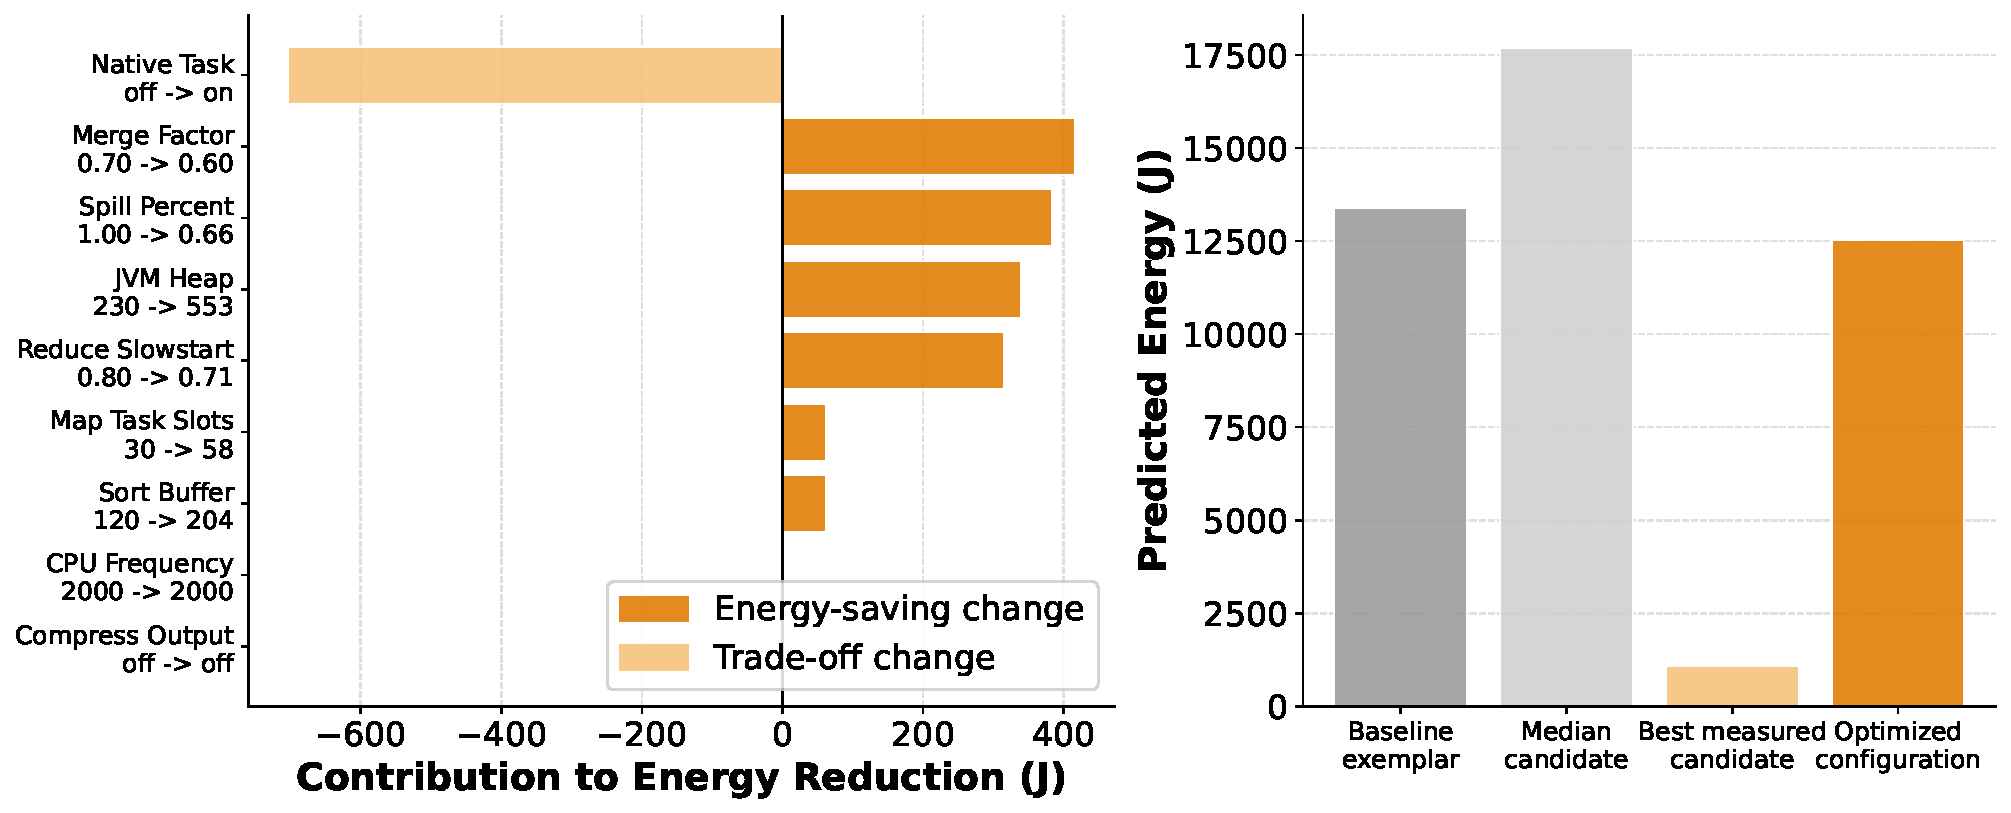
\includegraphics[width=\textwidth]{figures/parameter_attribution.pdf}
  \caption{NNBench 上的参数归因结果。橙色表示降低预测能耗的参数变化，浅橙色表示存在权衡的参数变化。}
  \label{fig:param_attribution}
\end{figure}

表~\ref{tab:param_attribution} 汇总了六个原始 benchmark 中主要的正向参数贡献。
可以看到，优化收益并非来自单一参数，而是由多个参数共同贡献。
例如，在 NNBench 中，主要正向贡献来自 Merge Factor、Spill Percent 和 JVM Heap 的调整；
这说明优化器并不是简单依赖一个较差 baseline，而是在多个 Hadoop 运行时参数之间寻找能耗和性能的折中。

\begin{table}[t]
  \centering
  \small
  \caption{六个原始 benchmark 中主要正向参数变化及其 Shapley 能耗贡献}
  \label{tab:param_attribution}
  \begin{tabularx}{\textwidth}{lYrrr}
    \toprule
    Benchmark & 参数变化 & Baseline & Optimized & 贡献 (J) \\
    \midrule
    TeraSort & Compress Output & on & off & 1122.4 \\
             & Sort Buffer & 110 & 183 & 967.3 \\
             & Map Task Slots & 10 & 47 & 631.9 \\
    \addlinespace
    PiEstimator & Native Task & off & on & 288.3 \\
                & JVM Heap & 320 & 999 & 277.6 \\
                & Reduce Slowstart & 0.70 & 0.90 & 156.0 \\
    \addlinespace
    PageRank & CPU Frequency & 3200 & 2200 & 3230.8 \\
             & Sort Buffer & 230 & 214 & 0.9 \\
             & JVM Heap & 420 & 615 & 0.9 \\
    \addlinespace
    Sort & Compress Output & on & off & 1460.1 \\
         & Reduce Slowstart & 0.50 & 0.69 & 1021.0 \\
         & Spill Percent & 0.62 & 0.64 & 108.6 \\
    \addlinespace
    Grep & JVM Heap & 750 & 550 & 34.4 \\
         & Map Task Slots & 30 & 53 & 15.6 \\
         & Sort Buffer & 200 & 197 & 2.1 \\
    \addlinespace
    NNBench & Merge Factor & 0.70 & 0.60 & 416.8 \\
            & Spill Percent & 1.00 & 0.66 & 384.0 \\
            & JVM Heap & 230 & 553 & 339.9 \\
    \bottomrule
  \end{tabularx}
\end{table}

\section{可放入 rebuttal 的说明}

我们新增了参数归因实验，以排除性能提升仅来自 poorly tuned baseline 的可能性。
具体而言，我们在原始六个 benchmark 上选择与端到端实验优化前能耗最接近的真实候选配置作为 baseline，
并对 baseline 到优化配置之间的九个参数变化计算精确 Shapley 值。
该过程枚举全部 \(2^9\) 个混合配置，并使用已训练的 CPU/IO 模型和 active-power 模型评估能耗。
结果显示，NNBench 中主要正向贡献来自 Merge Factor、Spill Percent 和 JVM Heap；
其他 benchmark 也表现出类似的多参数协同优化现象。
因此，观察到的收益不是简单来自一个任意差的 baseline，而是来自优化器对具体 Hadoop 参数和 CPU 频率的联合调整。

\end{document}
